\subsection{Калибровка точного времени (Fine time calibration)}

Пример таблицы калибровки точного времени, полученной на данных лабораторных тестов, представлен в виде графика на рисунке \ref{fig:TypicalCalibTable}. (Отметить, что не важно, какие данные.) По оси абсцисс откладывается значение счётчика точного времени, а по оси ординат --- значение точного времени в наносекундах. Обратим внимание, что в диапазоне значений десятибитного счетчика точного времени интервалу равному периоду грубого счетчика, т.е. 5 нс, соответствуют отсчеты от 30 до ???. Точные границы интервала определяются тем, что задержки на каждой ступени индивидуальны и зависят от флуктуаций технологического процесса.

С целью понимания особенностей работы счетчиков точного времени, каждая таблица калибровки точного времени была фитирована кусочно-линейной функцией. На рисунке \ref{fig:CalibTableMinusLinear} показан пример разности значений функции калибровки точного времени и линейной функции. Видно, что отклонения не превышают 60 пс.

%Заменить картинку

Параметры линейных функций для всех каналов отображены на двумерной гистограмме, рис. \ref{fig:ABmap}. Видно, что распределение хотя и двугорбое, но достаточно компактное.

Влияние замены точной функции калибровки на приближенную можно увидеть при одновременной оцифровке на нескольких каналах ВЦП сигналов с высокоточного генератора прямоугольных импульсов.
(Сначала нужно сказать, что для оценки качества калибровки необходимо исследовать одновременные фронты, которые можно получить от высокоточного генератора прямоугольных импульсов.)
(Расписать подробно ряд: точная калибр., индивид. линейная функция, глоб линейная функция, отсутствии калибр.)

В процедуре калибровки для каждого канала была выполнена замена калибровочной таблицы сначала индивидуальной линейной функцией данного канала, а потом усредненной. Полученные распределения разностей времен в исследуемом канале и в опорном показаны на рис \ref{}. (На самом деле ToT)
%Рисунок - Log 4 ToT
Видно, что полноценная калибровка точного времени необходима для достижения предельной точности ВЦП, составляющей ??? пс (FWHM). Использование индивидуальной линейной функции приводит к падению точности до ???, а усредненной --- до ??? (без калибровки) в наиболее неблагоприятных каналах.
Таким образом, при невозможности выполнить калибровку точного времени, например, из-за недостаточного массива данных, предоставленных для анализа, в условиях нашей задачи, когда характерное временное разрешение составляет несколько сотен пикосекунд, возможно применение усредненной линейной функции без заметного снижения точности.

\begin{figure}
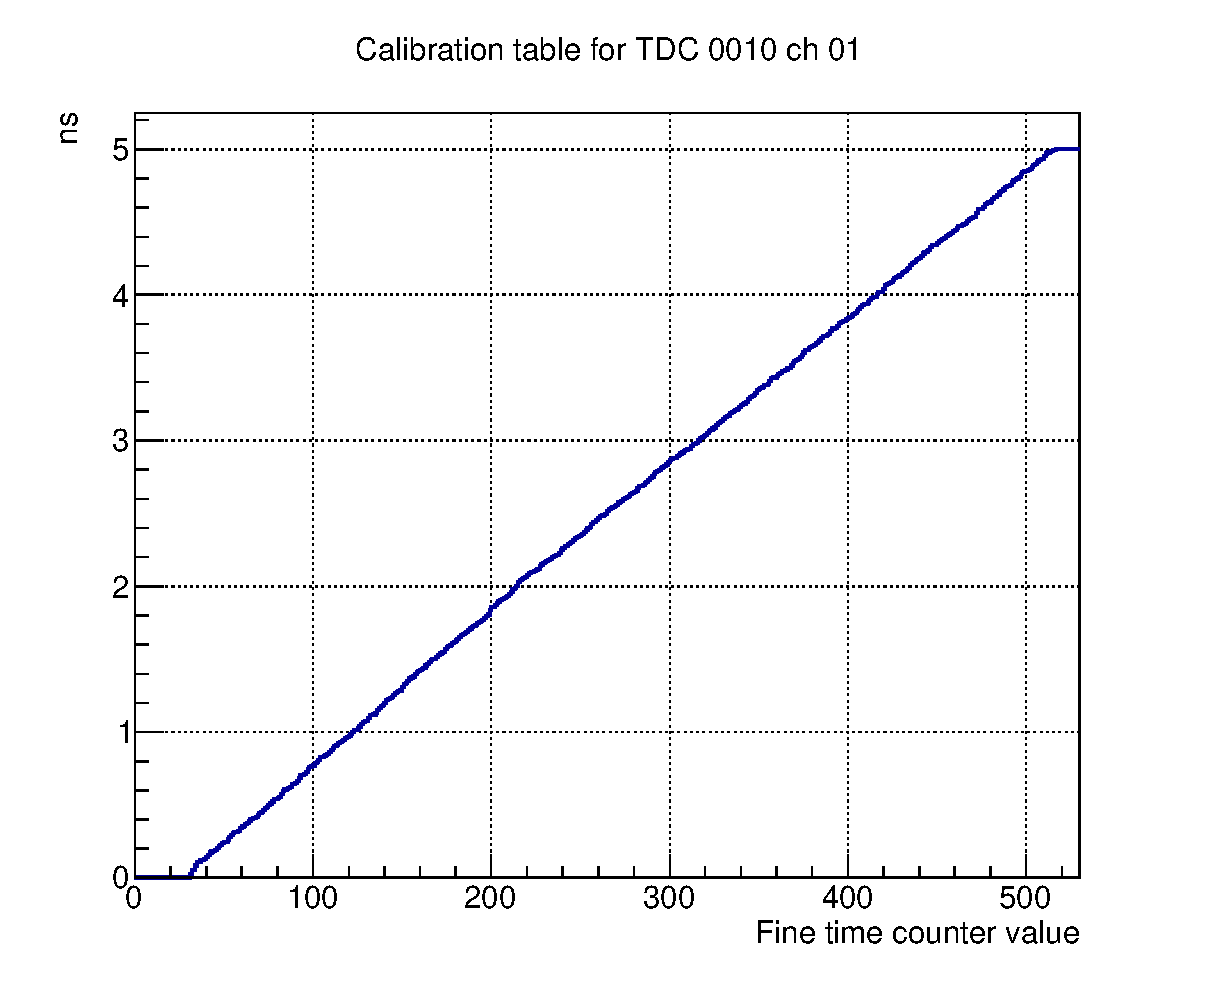
\includegraphics[width=1.0\textwidth]{pictures/Calib_table_example.eps}
\caption{Пример калибровочной кривой.}
\label{fig:TypicalCalibTable}
\end{figure}

\begin{figure}
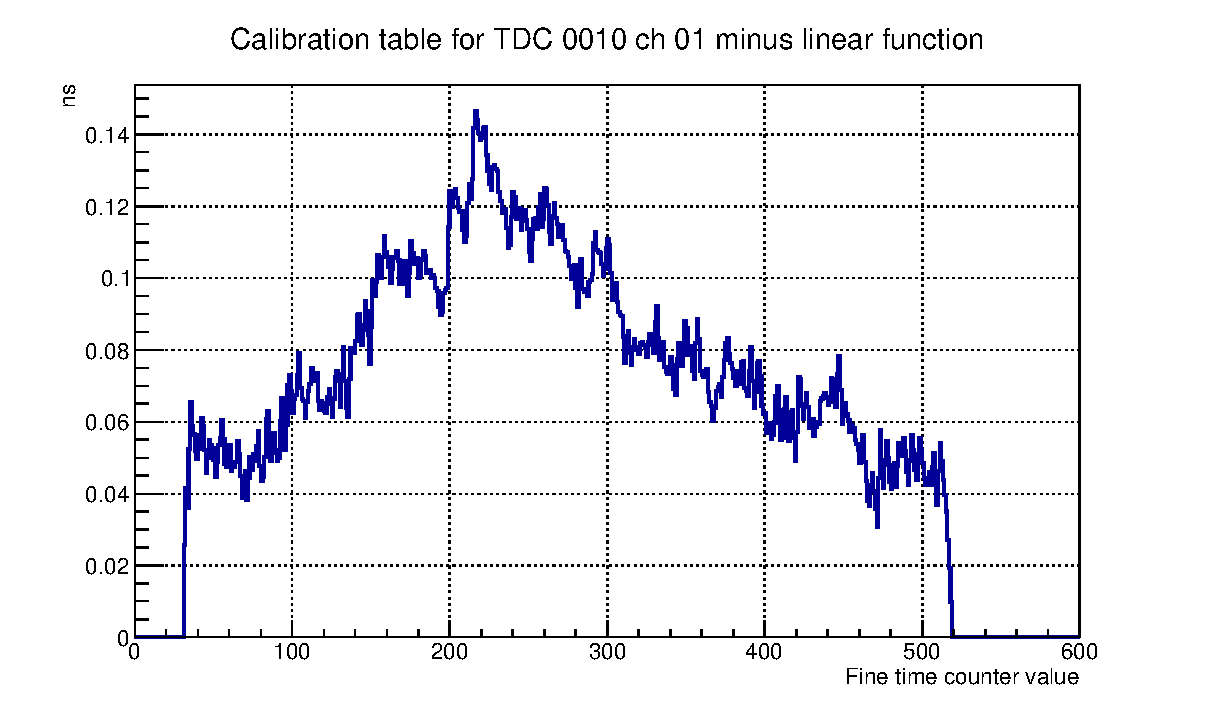
\includegraphics[width=1.0\textwidth]{pictures/CalibTable_minus_linear_0-600.eps}
\caption{Отклонение калибровочной кривой от линейной функции.}
\label{fig:CalibTableMinusLinear}
\end{figure}

\begin{figure}
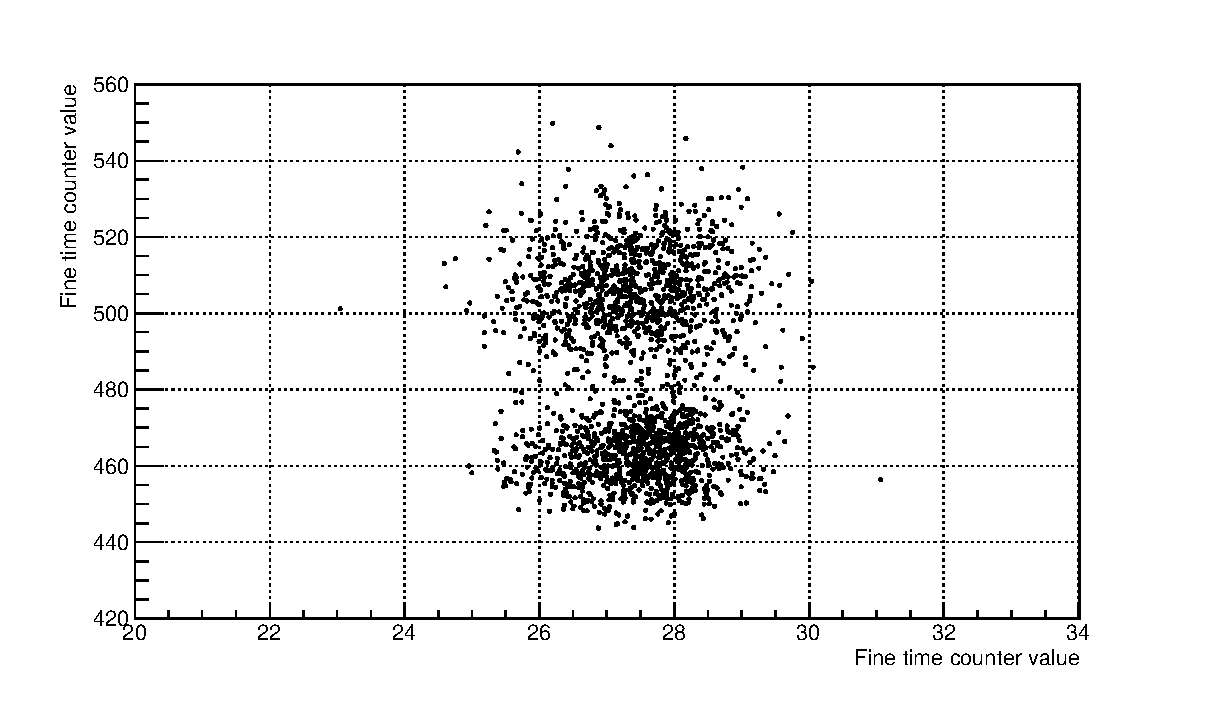
\includegraphics[width=1.0\textwidth]{pictures/ABmap.eps}
\caption{Распределение ????????. (описать понятно смысл параметров)}
\label{fig:ABmap}
\end{figure}



Приведенные выше функции калибровки были построены по массиву данных, содержащихся в семи файлах. Каждый файл это 2 минуты измерений при частоте генератора 5 кГц, т. е. около 600 тысяч вспышек лазера. Таким образом, всего было 4.2 миллиона вспышек за 14 минут, а один файл составляет приблизительно 15\% от полного набора данных. В каждом канале было зарегистрировано от 300 до 400 тысяч временных отметок, которые были использованы для выполнения калибровки. Для иллюстрации стабильности калибровки на рис. \ref{fig:Stability} показана разность функций калибровки, построенных по всему массиву данных и функций, построенных на файлах, составляющих $ \approx $15\% данных каждый, взятых в начале, середине и конце набора данных. Видно, что отклонения в основном не превышают 10 пс, однако имеются редкие выбросы до 20 пс.

%\begin{figure}
%\includegraphics[width=1.0\textwidth]{pictures/}
%\caption{Стабильность калибровок.}
%\label{fig:Stability}
%\end{figure}